\section{Experimental Design and Evidence}\label{sec:experiments}

\subsection{Experimental roadmap}\label{sec:exp-roadmap}
The experiments follow the argument developed in the theory.  E1 isolates the path-dependent reference mechanism and its decision consequence.  E2 then defines the shared semi-synthetic market setup and evaluates gradient estimation at fixed targets within that setup.  E3 releases the same setup as a continuous slow-variation online process and tests whether continued policy updates track the moving first-order target.  E4 perturbs the reference dynamics, episode horizon, and optimizer scale around the frozen E3 configuration to determine whether the tracking advantage occupies a parameter region rather than a single operating point.  \Cref{fig:evidence-map} summarizes this evidence chain; E5--E7 are reserved for real-market performance, investor behavior, and heterogeneous-agent interaction.

\begin{figure}[t]
    \centering
    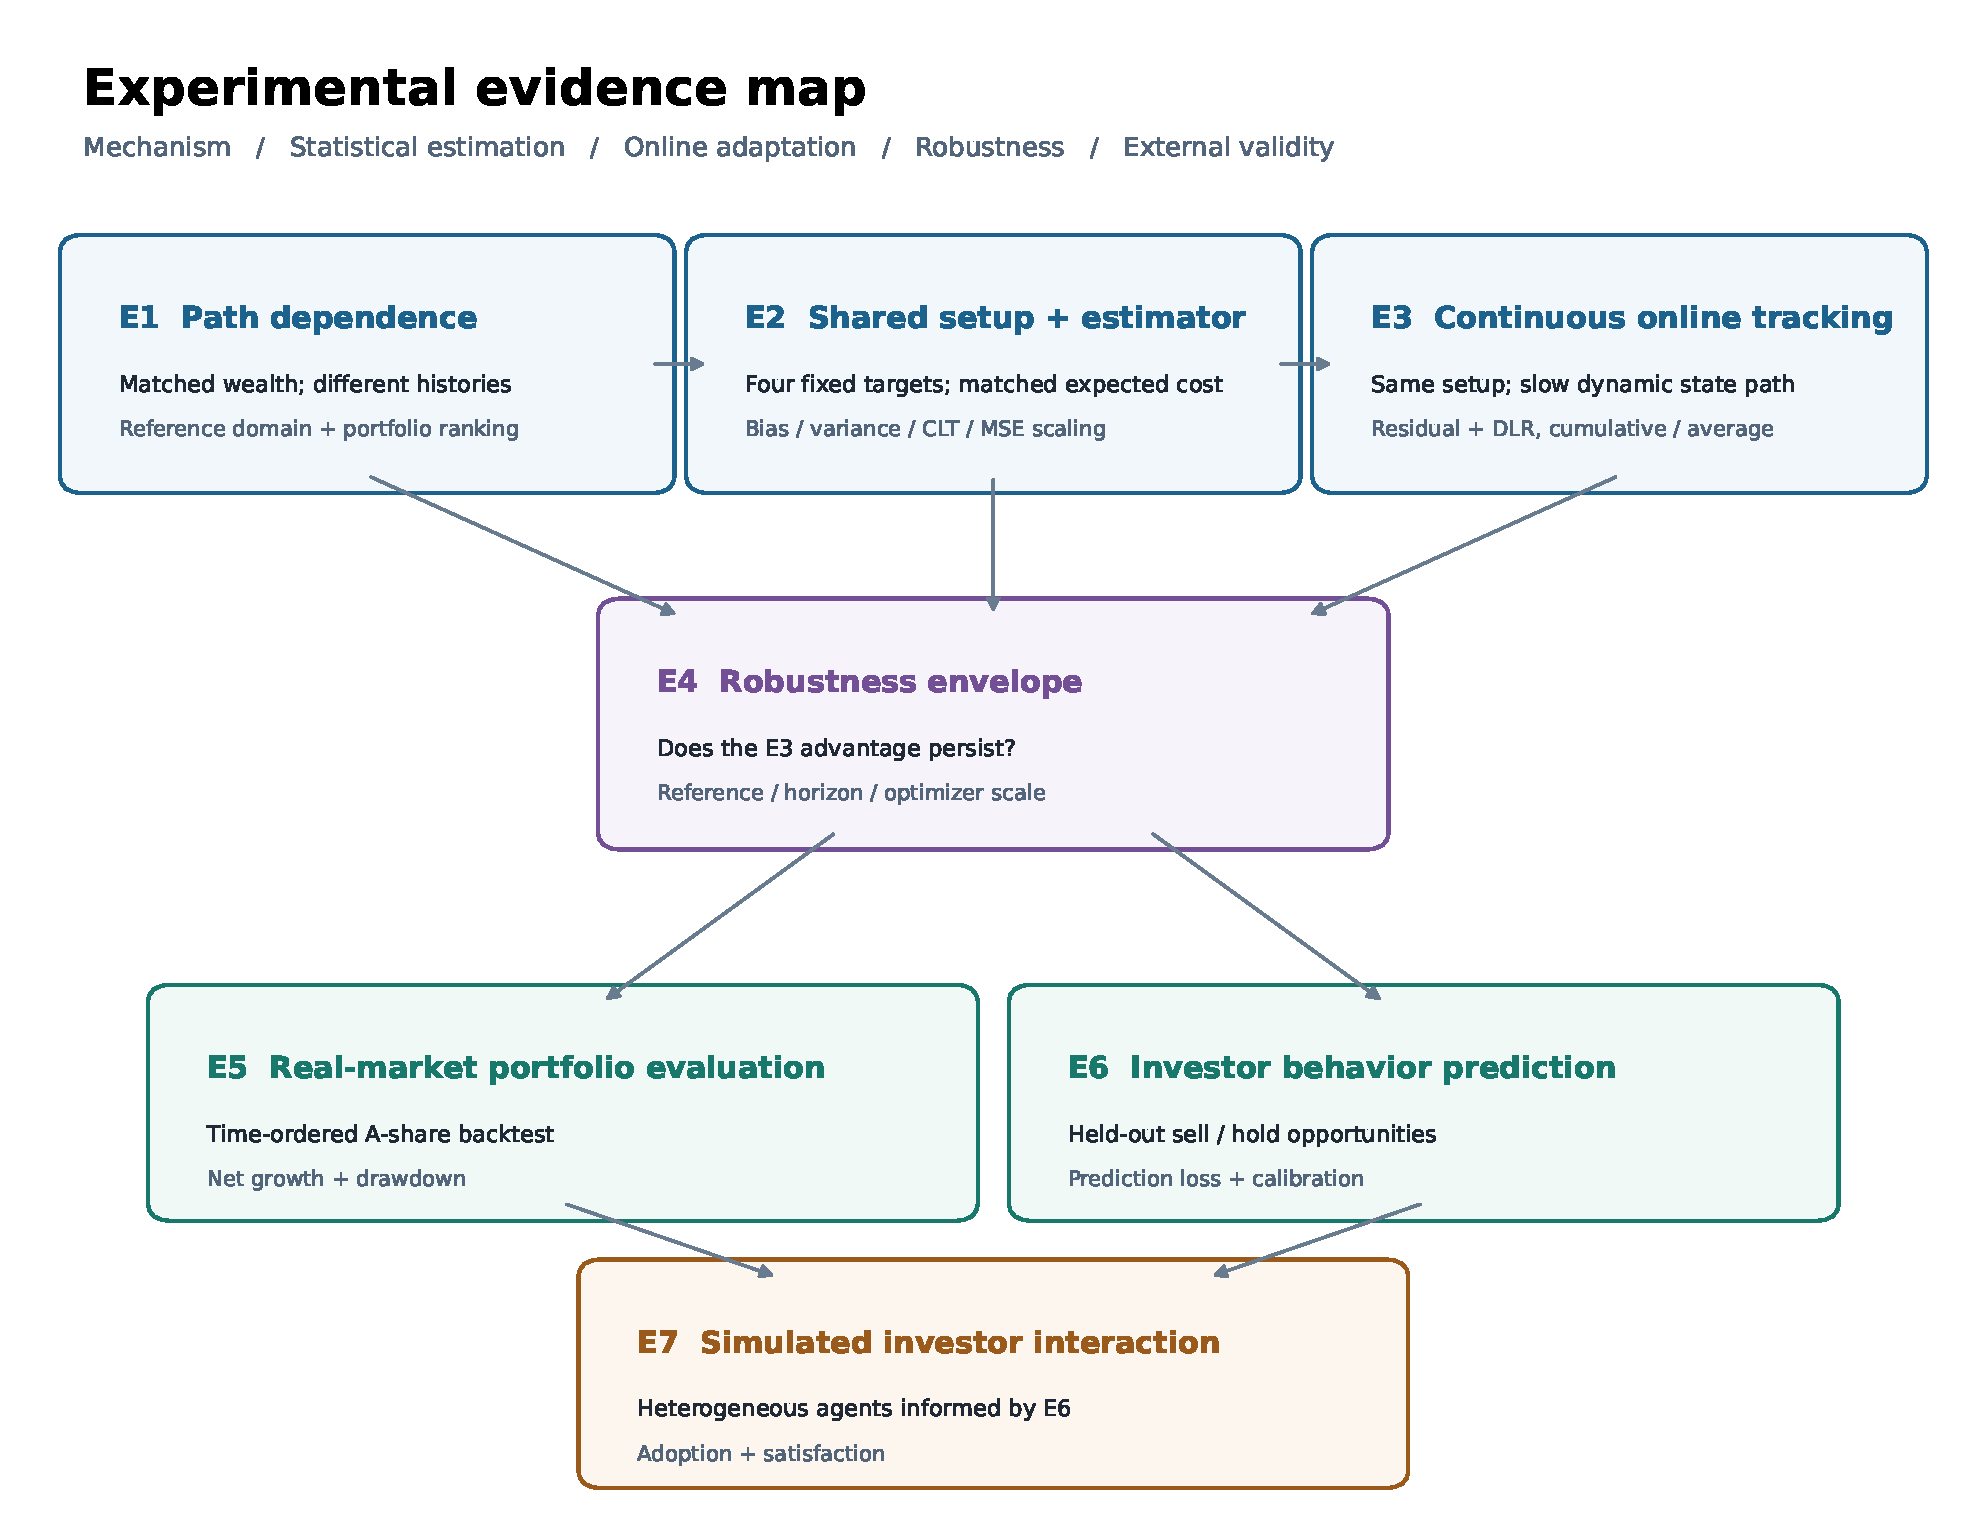
\includegraphics[width=0.96\textwidth]{figures/experiment_evidence_map.pdf}
    \caption{Experimental evidence map.  E1 establishes the decision consequence of path-dependent reference formation.  E2 evaluates the proposed gradient estimator at fixed targets in the shared semi-synthetic setup.  E3 runs the same setup continuously under a theory-aligned slow-variation construction and measures first-order tracking by projected residual and dynamic local regret (DLR).  E4 maps the robustness of the resulting online-tracking advantage.}
    \label{fig:evidence-map}
\end{figure}
\FloatBarrier

\subsection{E1: Path dependence and portfolio choice}\label{sec:e1}
\paragraph{Design.}
We construct two histories with the same initial wealth and the same endpoint,
\[
(1,1.10,1.015)
\qquad\text{and}\qquad
(1,0.90,1.015),
\]
and apply the reference recursion in \eqref{eq:reference-update} with $(\eta_+,\eta_-)=(0.20,0.05)$.  The histories are matched at the decision time: current wealth is $X_T=1.015$, the pre-trade portfolio is $50\%$ cash and $50\%$ risky asset, and the next risky return is $+4\%$ with probability $p$ and $-4\%$ otherwise.  We compare two feasible target allocations, $20\%$ and $80\%$ risky.  Under the action inertia in \eqref{eq:action-map}, these targets execute as $44\%$ and $56\%$ risky.  Because the next-period distribution has two states, all CPT values are evaluated exactly rather than by Monte Carlo.

\begin{figure}[t]
    \centering
    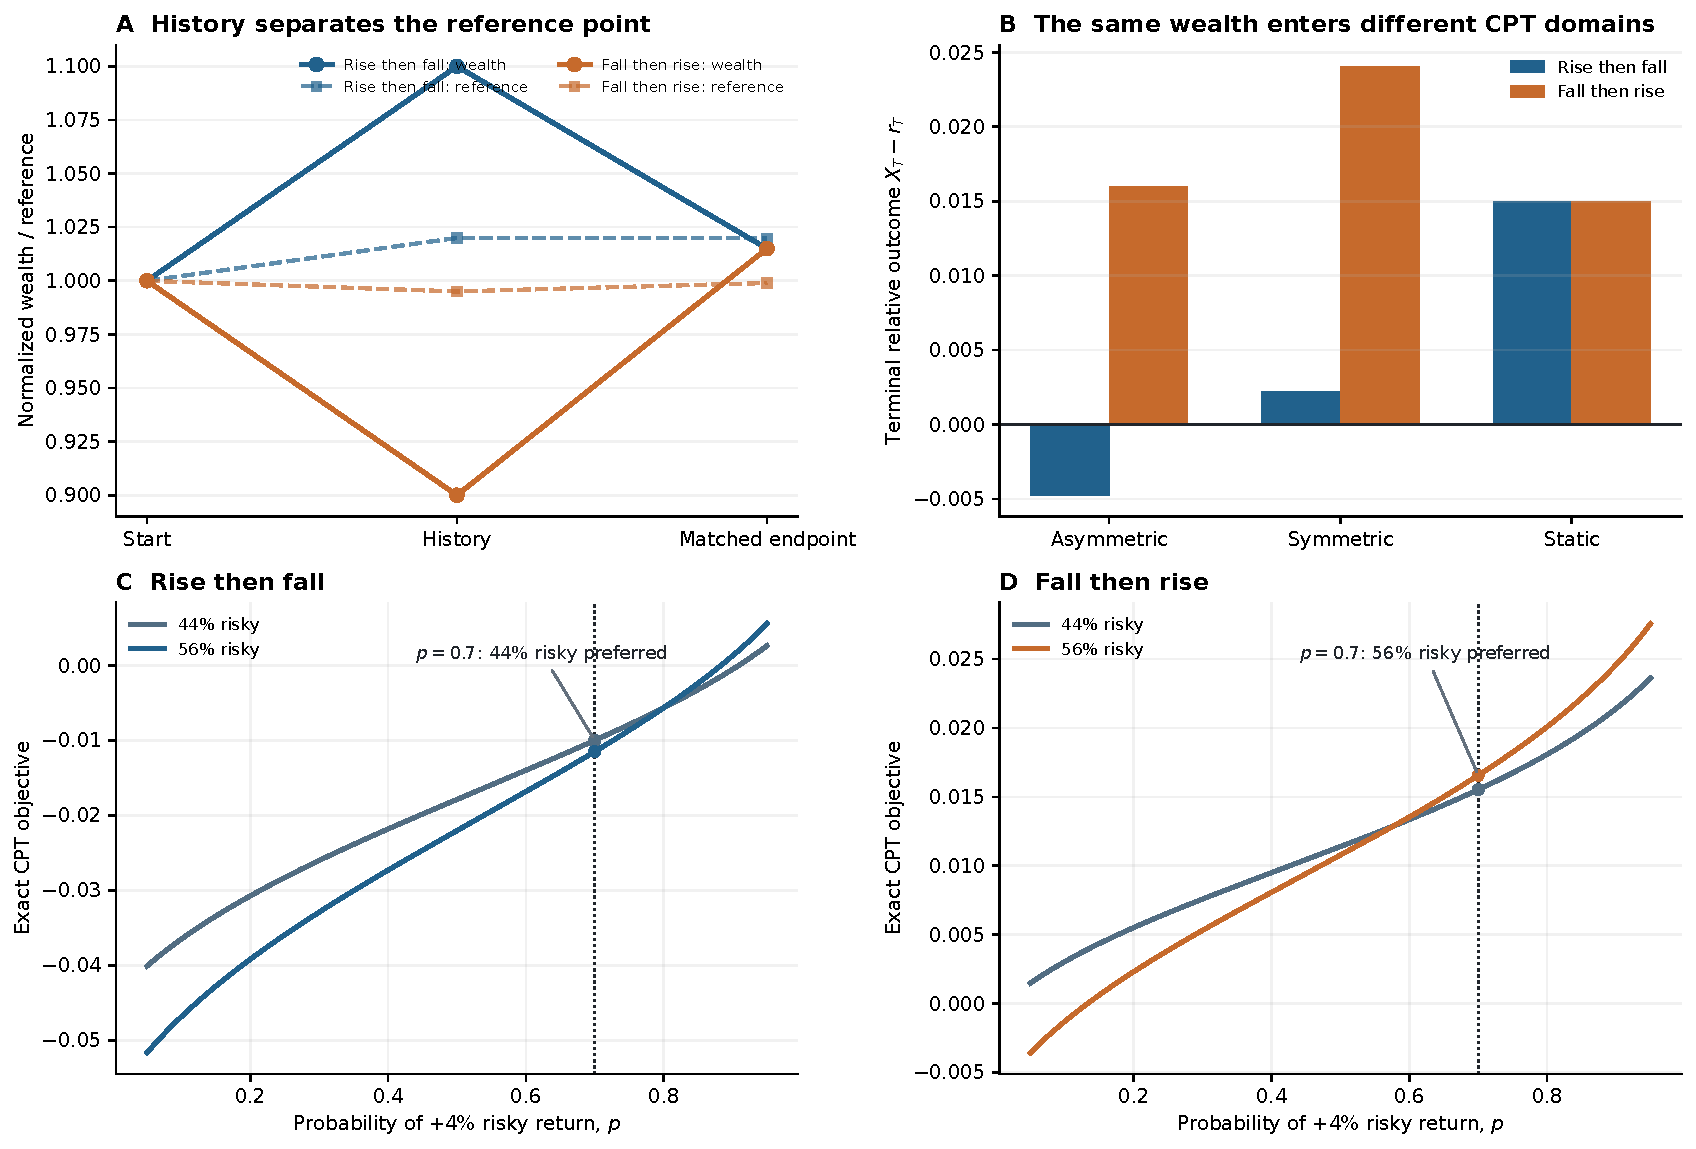
\includegraphics[width=\textwidth]{figures/e1_path_and_decision_final.pdf}
    \caption{Path dependence changes both the perceived domain and the portfolio ranking.  \textbf{A}: The two histories end at the same wealth but generate different asymmetric reference points.  \textbf{B}: The asymmetric rule places the rise--fall history below its reference and the fall--rise history above its reference; the symmetric and static rules provide mechanism controls.  \textbf{C--D}: Exact CPT values of the two feasible executed allocations as the probability $p$ of a $+4\%$ risky return varies.  At $p=0.7$, the matched rise--fall account prefers $44\%$ risky whereas the matched fall--rise account prefers $56\%$ risky.}
    \label{fig:e1-path-choice}
\end{figure}

\begin{table}[t]
\centering
\caption{E1 exact mechanism summary at $p=0.7$.}
\label{tab:e1-summary}
\begin{tabular}{lrrrrl}
\toprule
History & $X_T$ & $r_T$ & $X_T-r_T$ & Preferred risky share & CPT domain \\
\midrule
Rise then fall & 1.015 & 1.01975 & $-0.00475$ & 44\% & Loss \\
Fall then rise & 1.015 & 0.99900 & $+0.01600$ & 56\% & Gain \\
\bottomrule
\end{tabular}
\end{table}
\FloatBarrier

\paragraph{Results.}
The same terminal wealth is evaluated on opposite sides of the CPT reference.  After the rise--fall history, the reference is $1.01975$, so $X_T-r_T=-0.00475$; after the fall--rise history it is $0.999$, so $X_T-r_T=0.016$.  The separation propagates to the decision itself.  At $p=0.7$, the rise--fall history gives CPT values $-0.01001$ and $-0.01151$ for the $44\%$ and $56\%$ risky allocations, respectively, while the fall--rise history gives $0.01552$ and $0.01656$.  Thus two investors with identical current wealth, holdings, and opportunity set rank the same feasible portfolios differently solely because their histories imply different reference points.  This is the decision-level consequence of the path dependence characterized in \Cref{prop:path-dependence}.
\FloatBarrier

\subsection{E2: Finite-sample gradient estimation}\label{sec:e2}
\paragraph{Shared semi-synthetic setup.}
Beginning with E2, we use a common $30$-stock-plus-cash semi-synthetic market built from a frozen empirical A-share factor-block library.  Factor blocks are sampled from a time-invariant empirical distribution, while the return law follows a pre-specified path across episodes.  For risky asset $i$ in episode $k$,
\[
R_{i,k,u}=0.08\,\tanh\!\left(
\frac{\mu_k+2.5\,b_k^\top f_{i,u}+\xi^{\rm com}_{k,u}+\xi^{\rm id}_{i,k,u}}{0.08}
\right),
\]
where the common and idiosyncratic shocks have standard deviations $0.006s_k$ and $0.009s_k$, respectively.  Episodes $1$--$40$ use the stable momentum law, episodes $41$--$60$ use the reversal law, episodes $61$--$120$ interpolate to the terminal low-volatility/value/quality law, and the exogenous return law is fixed thereafter.  E2 standardizes the account context to
\[
(X,r,\omega,\theta)=(1,1,e_{\rm cash},0)
\]
and freezes four pre-specified targets at episodes $20$, $50$, $90$, and $150$, corresponding to the stable, post-change, mid-drift, and post-drift phases.  E3 subsequently uses the same factor distribution and episode-specific return law but allows the account state to evolve continuously.

We compare the proposed centered leave-one-out estimator with independent raw randomized correction against the raw independent-split plug-in estimator used by the adapted CPT-PG v5 baseline.  Both target the square-smoothed CPT objective in \eqref{eq:value-functions}.  Expected complete-trajectory cost is matched over
\[
\mathsf B\in\{32,64,128,256,512,1024,2048\},
\]
and numerical gradient references are generated independently at substantially higher cost.

\begin{figure}[t]
    \centering
    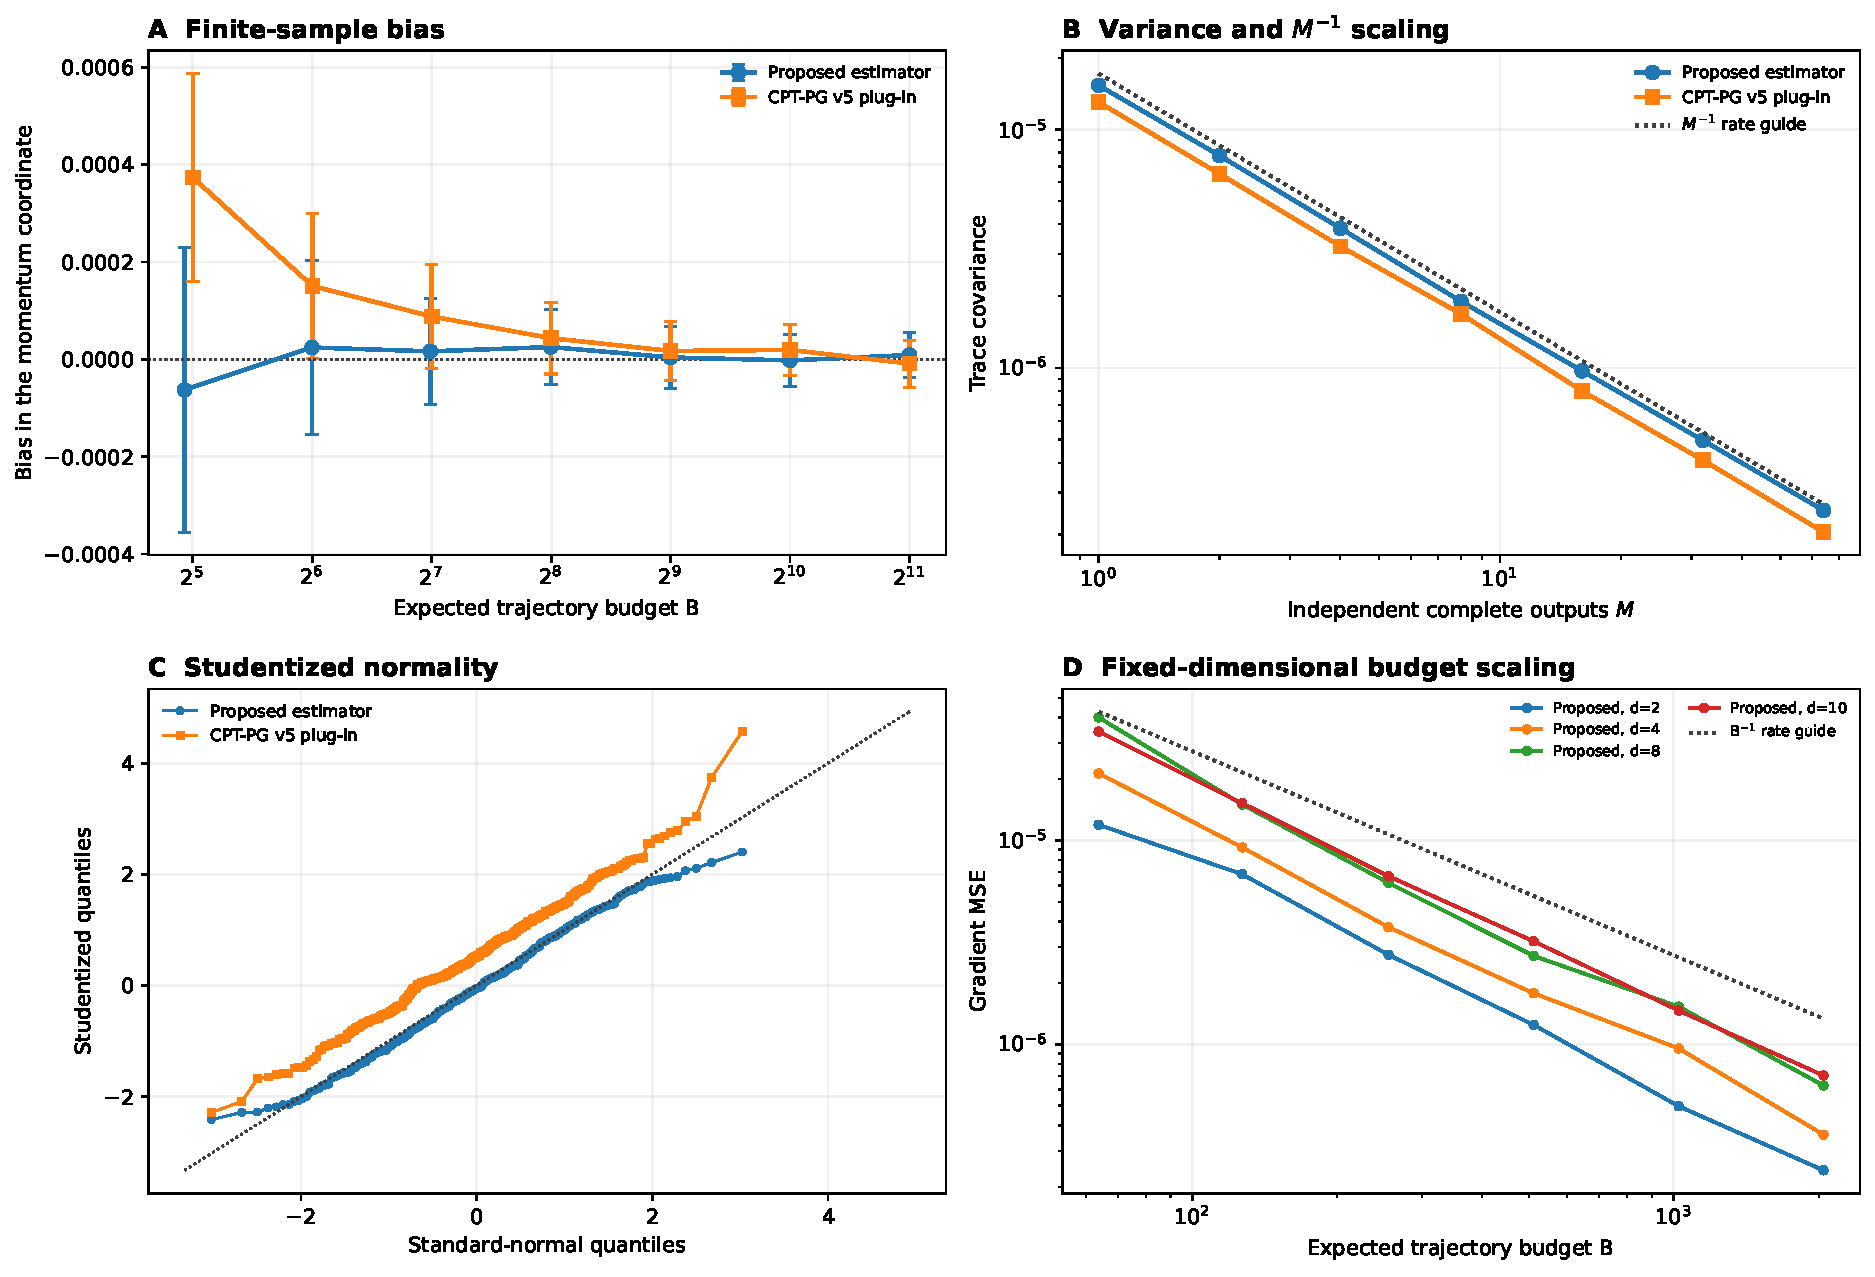
\includegraphics[width=\textwidth]{figures/e2_estimator_diagnostics.pdf}
    \caption{Finite-sample gradient estimation in the shared semi-synthetic setup.  \textbf{A}: coordinate bias at the stable target.  \textbf{B}: trace covariance of averages of $M$ independent complete estimator outputs; the dotted reference has slope $-1$.  \textbf{C}: studentized normal-quantile diagnostic at $M=64$.  \textbf{D}: full-gradient MSE versus expected trajectory budget for $d\in\{2,4,8,10\}$; the dotted reference has slope $-1$.  The corresponding unbiasedness, asymptotic normality, and fixed-dimensional minimax statements are given in \Cref{thm:estimator,thm:clt,thm:minimax}.}
    \label{fig:e2-estimator}
\end{figure}

\begin{table}[t]
\centering
\small
\caption{Full-gradient MSE at expected trajectory budget $\mathsf B=512$ across the four fixed targets.  MSE entries are in units of $10^{-6}$.  The last column gives a paired 95\% bootstrap interval for $\mathrm{MSE}_{\rm prop}-\mathrm{MSE}_{\rm v5}$ in the same units.}
\label{tab:e2-period-mse}
\begin{tabular}{lrrrr}
\toprule
Target & Proposed & CPT-PG v5 & Ratio & Difference 95\% CI \\
\midrule
Stable & 3.123 & 2.938 & 1.063 & $[-0.055,\ 0.434]$ \\
Post-change & 10.134 & 10.809 & 0.938 & $[-1.495,\ 0.139]$ \\
Mid-drift & 10.647 & 11.468 & 0.928 & $[-1.739,\ 0.102]$ \\
Post-drift & 10.589 & 12.257 & 0.864 & $[-2.599,-0.721]$ \\
\bottomrule
\end{tabular}
\end{table}
\FloatBarrier

\paragraph{Results.}
The four diagnostics separate estimator centering from ordinary Monte Carlo variance.  At the stable target, the proposed coordinate estimate remains centered near the numerical reference across the budget range, while the plug-in estimator exhibits the larger low-budget displacement expected from nonlinear probability weighting (\Cref{fig:e2-estimator}A).  Once independent complete outputs are averaged, both estimators recover the predicted inverse-replication variance rate: the fitted log--log slopes are $-0.989$ for the proposed estimator and $-0.999$ for CPT-PG v5 (\Cref{fig:e2-estimator}B).  The proposed estimator also exhibits inverse-budget full-gradient MSE across $d=2,4,8,10$, with slopes between $-1.17$ and $-1.12$, consistent with the fixed-dimensional $\Theta(\mathsf B^{-1})$ rate in \Cref{thm:minimax}.

The studentized outputs sharpen the centering comparison.  At $M=64$, the proposed statistic has mean $-0.049$, standard deviation $0.993$, and 95\% coverage of $96.25\%$, whereas the v5 statistic has mean $0.556$ and coverage of $91.75\%$ (\Cref{fig:e2-estimator}C).  At the standard budget $\mathsf B=512$, the proposed estimator has the lower MSE point estimate in three of the four fixed targets; the post-drift reduction is $13.6\%$ and its paired interval lies entirely below zero (\Cref{tab:e2-period-mse}).  Thus the debiased construction preserves the expected $1/\mathsf B$ statistical rate while improving finite-sample centering and delivering competitive or lower full-gradient error across the pre-specified market states.
\FloatBarrier

\subsection{E3: Continuous slow-variation online tracking}\label{sec:e3}
\paragraph{Design.}
E3 releases the market setup introduced in E2 as one continuous online process.  No account state is reset.  If a five-day episode starting from $(X_k,r_k,\omega_k)$ produces the raw terminal state $(\widetilde X_{k+1},\widetilde r_{k+1},\widetilde\omega_{k+1})$, the next episode starts from the diminishing-gain transition
\[
\begin{aligned}
\log X_{k+1}
&=(1-\alpha_k)\log X_k+\alpha_k\log\widetilde X_{k+1},\\
r_{k+1}
&=(1-\alpha_k)r_k+\alpha_k\widetilde r_{k+1},\\
\omega_{k+1}
&=(1-\alpha_k)\omega_k+\alpha_k\widetilde\omega_{k+1},
\qquad
\alpha_k=k^{-3/4}.
\end{aligned}
\]
The within-episode reference update remains the asymmetric mechanism in \eqref{eq:reference-update} with $(\eta_+,\eta_-)=(0.20,0.05)$.  Hence the reference point retains its cross-episode memory, while bounded raw transitions imply episode-start state increments of order $O(\alpha_k)$ and
\[
\sum_{k\le K}\alpha_k=O(K^{1/4})=o(K).
\]
The factor-block distribution is time invariant, the exogenous return coefficients follow the E2 phase path through episode $120$, and remain fixed for episodes $121$--$300$.  This construction keeps the dynamic-reference system continuous while imposing a sublinear state-step budget, providing the theory-aligned slow-variation setting used to probe \Cref{cor:vanishing-tracking}.

The comparison uses $20$ independent test trajectories.  The online learner and frozen control share the complete path through episode $40$.  Thereafter the online learner continues Algorithm~\ref{alg:drcptpg}, whereas the control freezes $\theta$ but continues to propagate wealth, reference, and holdings under the same slow transition.  We fix $(\gamma,\vartheta)=(0.08,0.05)$ before the E3 test runs and use the growing replication schedule
\[
M_k=\max\{4,\lceil\sqrt{k}\rceil\},
\]
so that the average inverse replication count decays as $O(K^{-1/2})$ by \eqref{eq:growing-replication-bound}.  DLR follows \eqref{eq:dynamic-regret} with $w=5$ and $\rho=0.9$.  Two independent evaluation streams estimate both the projected residual and the windowed squared residual by cross-stream products, preventing the ordinary self-square noise term from entering the evaluation.

\begin{figure}[t]
    \centering
    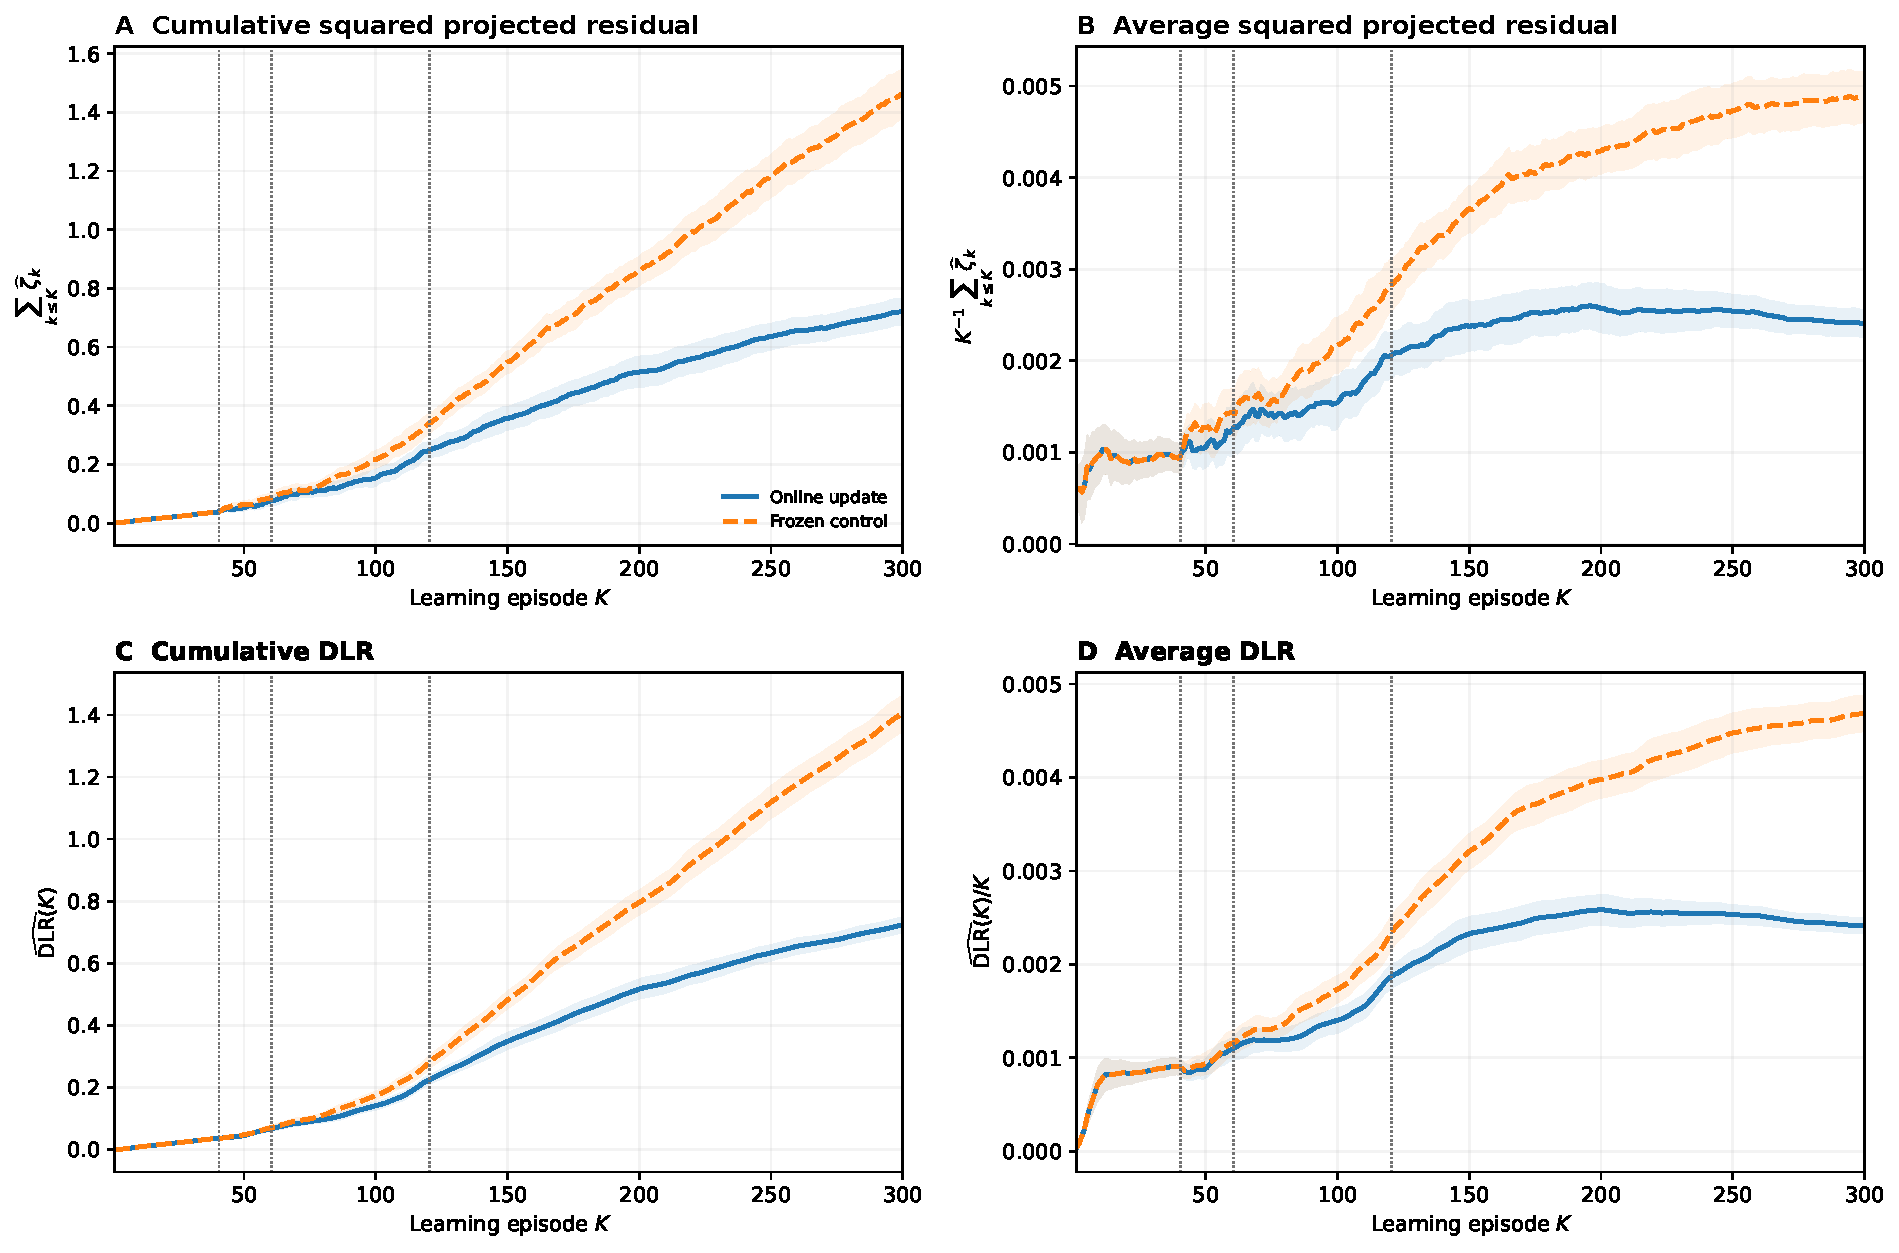
\includegraphics[width=\textwidth]{figures/e3_online_tracking.pdf}
    \caption{Continuous online tracking under slow variation.  \textbf{A--B}: cumulative and average projected residual.  \textbf{C--D}: cumulative and average DLR.  The two methods share the same trajectory through episode $40$; thereafter the frozen control holds $\theta$ fixed while both methods continue to propagate their own wealth, reference, and holdings.  Dotted lines mark the abrupt change, the start of gradual drift, and the point after which the exogenous return law is fixed.  Curves are means over $20$ independent trajectories and shaded bands are $1.96$ standard errors.}
    \label{fig:e3-tracking}
\end{figure}
\FloatBarrier

\paragraph{Results.}
Continued updating produces substantially lower closed-loop tracking accumulation than freezing the policy parameter after episode $40$.  Over episodes $41$--$300$, cumulative projected residual is $0.684$ for the online learner and $1.427$ for the frozen control, while cumulative DLR is $0.687$ versus $1.369$; the seed-paired differences have 95\% bootstrap intervals $[-0.834,-0.650]$ and $[-0.738,-0.622]$, respectively.  By episode $300$, average DLR is $2.411\times10^{-3}$ online and $4.685\times10^{-3}$ frozen (\Cref{fig:e3-tracking}D).  Because the policies induce different endogenous account paths after they diverge, the frozen curve is a closed-loop control rather than a common-objective optimizer comparison.  The direct theory-aligned diagnostic is therefore the evolution of the online residual and DLR along its own moving objective sequence.

The slow-variation tail also changes the growth rate of accumulated tracking error.  Over episodes $121$--$300$, the empirical log--log slope of cumulative DLR is $0.704$ for continued updating and $0.968$ for the frozen control; the corresponding projected-residual slopes are $0.745$ and $0.959$.  The online exponent below one is consistent with the sublinear direction predicted by \Cref{cor:dynamic-local-regret,cor:vanishing-tracking} for a slowly varying target sequence.  Under the optional error-bound condition in \Cref{ass:error-bound}, the online average projected residual also controls the average squared distance from its policy iterates to the contemporaneous stationary set through \Cref{cor:stationary-tracking}.
\FloatBarrier

\subsection{E4: Robustness of online tracking}\label{sec:e4}
\paragraph{Design.}
E4 tests whether the E3 closed-loop tracking advantage persists when the reference dynamics, decision horizon, and optimizer scale are perturbed.  Because each perturbation changes the induced objective sequence, absolute DLR values are not compared across configurations.  Instead, within each configuration $c$ we report the matched-control ratio
\[
\mathcal R_{\rm DLR}(c)
=\frac{\mathrm{DLR}^{\rm post}_{\rm online}(c)}{\mathrm{DLR}^{\rm post}_{\rm frozen}(c)},
\]
where the post-change interval begins at the first regime change.  This is a within-configuration normalization of the same DLR used in E3, not a new loss; $\mathcal R_{\rm DLR}<1$ means that continued updating accumulates less DLR than freezing $\theta$ under the same configuration.

Panel A evaluates the full $9\times9$ reference grid
\[
\eta_+,\eta_-\in\{0,0.05,0.10,\ldots,0.40\}.
\]
Panel B varies the episode horizon over
\[
h\in\{1,2,4,5,10,20,25,50\},
\]
while holding total market time at $1500$ days and tying the state-gain clock to elapsed market time.  Panel C evaluates $48$ admissible optimizer configurations from
\[
\gamma\in\{0.01,0.02,0.03,0.04,0.05,0.06,0.08,0.10,0.12\},
\]
\[
\vartheta\in\{0.005,0.01,0.015,0.02,0.03,0.04,0.05,0.06\},
\qquad
\gamma L_{\rm diag}\le\vartheta,
\quad L_{\rm diag}=0.31.
\]
The E3 defaults $(\eta_+,\eta_-)=(0.20,0.05)$, $h=5$, and $(\gamma,\vartheta)=(0.08,0.05)$ are marked but are not re-selected in E4.  Each configuration uses four independent paired trajectories.

\begin{figure}[H]
    \centering
    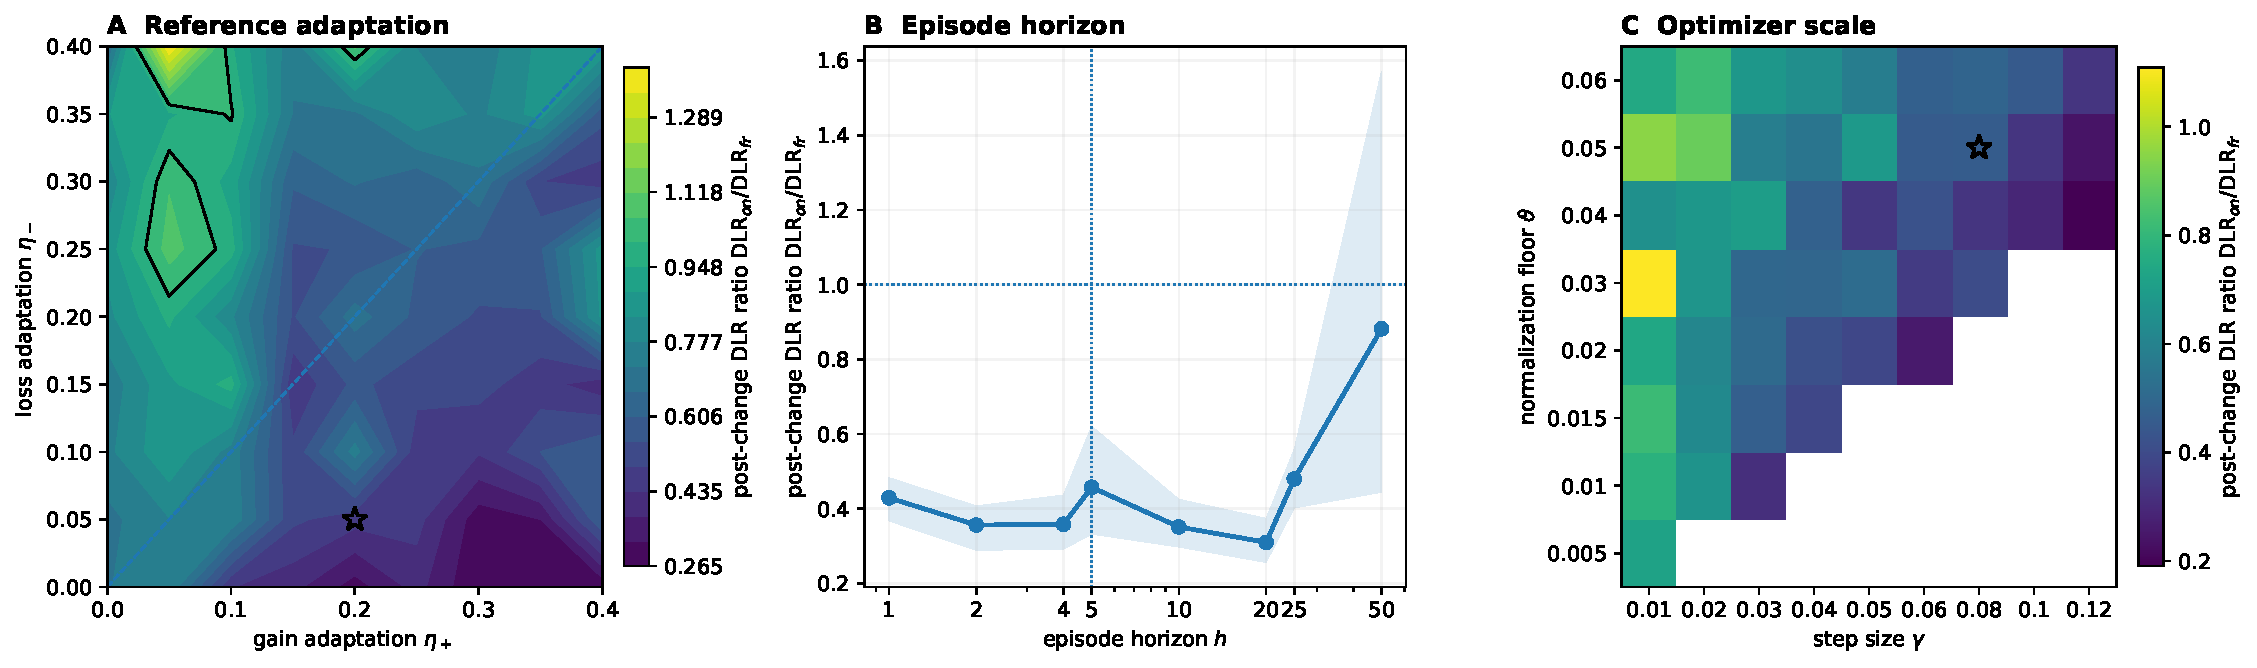
\includegraphics[width=\textwidth]{figures/e4_robustness.pdf}
    \caption{Robustness of the online-tracking advantage measured by the configuration-matched post-change DLR ratio $\mathcal R_{\rm DLR}$.  \textbf{A}: reference-adaptation surface over the simulated $9\times9$ grid; the black contour marks $\mathcal R_{\rm DLR}=1$, the diagonal marks $\eta_+=\eta_-$, and the star marks the default asymmetric rule.  \textbf{B}: horizon sweep with paired-seed 95\% bootstrap intervals; the horizontal line marks $\mathcal R_{\rm DLR}=1$ and the vertical line marks $h=5$.  \textbf{C}: admissible $(\gamma,\vartheta)$ grid; blank cells are excluded by $\gamma L_{\rm diag}>\vartheta$, and the star marks the E3 default.}
    \label{fig:e4-robustness}
\end{figure}
\FloatBarrier

\paragraph{Results.}
The reference-adaptation surface places most of the simulated grid below the matched-control boundary: $76$ of $81$ configurations have $\mathcal R_{\rm DLR}<1$, and $59$ have paired 95\% intervals entirely below one.  All $36$ asymmetric configurations with $\eta_+>\eta_-$ lie below one, including $33$ with intervals entirely below one.  At the default rule $(0.20,0.05)$, the mean ratio is $0.458$ with a 95\% interval $[0.332,0.621]$.  The only region that clearly reverses the comparison is strongly loss-dominant adaptation; for example, $(0.05,0.40)$ gives a ratio of $1.403$ with interval $[1.224,1.552]$ (\Cref{fig:e4-robustness}A).

The horizon sweep gives ratios below one at all eight tested horizons.  Seven intervals lie entirely below one; the ratio ranges from $0.310$ at $h=20$ to $0.882$ at $h=50$, where the interval widens to $[0.444,1.572]$ and includes the neutral boundary (\Cref{fig:e4-robustness}B).  The optimizer sweep shows the same broad pattern: $47$ of $48$ admissible configurations have mean ratios below one and $45$ have intervals entirely below one.  The single point estimate above one, $(\gamma,\vartheta)=(0.01,0.03)$, has interval $[0.876,1.342]$ and is not resolved from the matched control.  Together, the dense sweeps show that the E3 closed-loop tracking advantage extends over broad reference, horizon, and optimizer regions rather than depending on the default operating point.
\FloatBarrier

\subsection{E5: Real-market portfolio evaluation}\label{sec:e5}
\placeholder{Time-ordered A-share backtest with return, risk, turnover, and cost metrics.}

\subsection{E6: Investor behavior prediction}\label{sec:e6}
\placeholder{Held-out investor sell/hold prediction and calibration.}

\subsection{E7: Simulated heterogeneous-investor interaction}\label{sec:e7}
\placeholder{Repeated interaction with heterogeneous simulated investor agents.}
